% Options for packages loaded elsewhere
\PassOptionsToPackage{unicode}{hyperref}
\PassOptionsToPackage{hyphens}{url}
%
\documentclass[
]{article}
\author{}
\date{\vspace{-2.5em}}

\usepackage{amsmath,amssymb}
\usepackage[]{URW A030}
\usepackage{iftex}
\ifPDFTeX
  \usepackage[T1]{fontenc}
  \usepackage[utf8]{inputenc}
  \usepackage{textcomp} % provide euro and other symbols
\else % if luatex or xetex
  \usepackage{unicode-math}
  \defaultfontfeatures{Scale=MatchLowercase}
  \defaultfontfeatures[\rmfamily]{Ligatures=TeX,Scale=1}
\fi
% Use upquote if available, for straight quotes in verbatim environments
\IfFileExists{upquote.sty}{\usepackage{upquote}}{}
\IfFileExists{microtype.sty}{% use microtype if available
  \usepackage[]{microtype}
  \UseMicrotypeSet[protrusion]{basicmath} % disable protrusion for tt fonts
}{}
\makeatletter
\@ifundefined{KOMAClassName}{% if non-KOMA class
  \IfFileExists{parskip.sty}{%
    \usepackage{parskip}
  }{% else
    \setlength{\parindent}{0pt}
    \setlength{\parskip}{6pt plus 2pt minus 1pt}}
}{% if KOMA class
  \KOMAoptions{parskip=half}}
\makeatother
\usepackage{xcolor}
\IfFileExists{xurl.sty}{\usepackage{xurl}}{} % add URL line breaks if available
\IfFileExists{bookmark.sty}{\usepackage{bookmark}}{\usepackage{hyperref}}
\hypersetup{
  hidelinks,
  pdfcreator={LaTeX via pandoc}}
\urlstyle{same} % disable monospaced font for URLs
\usepackage[margin=1in]{geometry}
\usepackage{graphicx}
\makeatletter
\def\maxwidth{\ifdim\Gin@nat@width>\linewidth\linewidth\else\Gin@nat@width\fi}
\def\maxheight{\ifdim\Gin@nat@height>\textheight\textheight\else\Gin@nat@height\fi}
\makeatother
% Scale images if necessary, so that they will not overflow the page
% margins by default, and it is still possible to overwrite the defaults
% using explicit options in \includegraphics[width, height, ...]{}
\setkeys{Gin}{width=\maxwidth,height=\maxheight,keepaspectratio}
% Set default figure placement to htbp
\makeatletter
\def\fps@figure{htbp}
\makeatother
\setlength{\emergencystretch}{3em} % prevent overfull lines
\providecommand{\tightlist}{%
  \setlength{\itemsep}{0pt}\setlength{\parskip}{0pt}}
\setcounter{secnumdepth}{-\maxdimen} % remove section numbering
\usepackage{booktabs}
\usepackage{longtable}
\usepackage{array}
\usepackage{multirow}
\usepackage{wrapfig}
\usepackage{float}
\usepackage{colortbl}
\usepackage{pdflscape}
\usepackage{tabu}
\usepackage{threeparttable}
\usepackage{threeparttablex}
\usepackage[normalem]{ulem}
\usepackage{makecell}
\usepackage{xcolor}
\ifLuaTeX
  \usepackage{selnolig}  % disable illegal ligatures
\fi

\begin{document}

Data analyses was done in R v. 4.1.1. Various factors such as the effect
of sex and mating status were tested using various statiscal models.

\hypertarget{males-vs-females-experiment-1}{%
\subsection{Males vs Females (Experiment
1)}\label{males-vs-females-experiment-1}}

\hypertarget{feeding-behaviour}{%
\subsubsection{Feeding behaviour}\label{feeding-behaviour}}

A linear model was used and the significance of day was tested using an
ANOVA model. It was found that day was significant
(F\textsubscript{8,903} = 0.941, P = 0.05). ANOVA analysis also showed
that there was significance between the sexes and the interaction effect
(F\textsubscript{8,903} = 35.36, P = \textless0.001), so this was kept
in the model.

The significance of diets between sexes and within sexes was analysed.

There was a statistically significant difference found between a 1:2
diet and an 8:1 diet on the female assay on both day 1 and day 2 (Tukey
test: t\textsubscript{903} = -5.088, P \textless{} 0.001). On day 1, the
there was a mean average of 1.43 +/- S.E. 0.154 flies per patch but on
day 2 there was an average of 2.36 +/- S.E. 0.230 flies per patch on the
8:1 diet.

The significance of sex differences was analysed using a generalised
linear model with quasipoisson to count for overdispersion. It was found
that there was a significant difference in male and female flies
choosing a diet higher in protein (a 2:1 diet). A tukey test was used to
analyse this (t\textsubscript{903}8\textasciitilde{} = 13.048, P
\textless{} 0.001). Day was not considered in this model.

\hypertarget{mated-vs-virgin-females-experiment-2---feeding-and-oviposition-behaviour}{%
\subsection{Mated vs Virgin females (Experiment 2) - Feeding and
Oviposition
behaviour}\label{mated-vs-virgin-females-experiment-2---feeding-and-oviposition-behaviour}}

\hypertarget{feeding-behaviour-1}{%
\subsubsection{Feeding behaviour}\label{feeding-behaviour-1}}

A generalised linear model was used with quasipoisson to count for
overdispersion. Day was dropped from the model as there was found to be
no significant effect of including day in the model (ANOVA:
F\textsubscript{1,1159} = 0.8, P = 0.35). There was found to be a very
strong statistically significant effect however on the interaction of
diet and type (whether the fly was mated or virgin) (ANOVA:
F\textsubscript{3,1159} = 0.8, P = \textless{} 0.0001).

Post hoc analysis showed there were statistically significant
differences for the diets chosen between mated and virgin female
\emph{drosophila melanogaster}. Between the types of fly, there was a
significant difference in choosing a diet high in protein (8:1). (Tukey
test: z\textsubscript{1151} = 5.301, P \textless{} 0.001). With a mean
average of 2.74 +/- S.E. 0.138 mated females per patch and a mean
average of 1.64 +/- S.E. 0.146 virgin females. This shows that mated
females will prefer a diet which is high in protein, indicating that
mated females are sensible enough to chose a diet which is good for
pregnancy, contributing to the growth of their offspring.

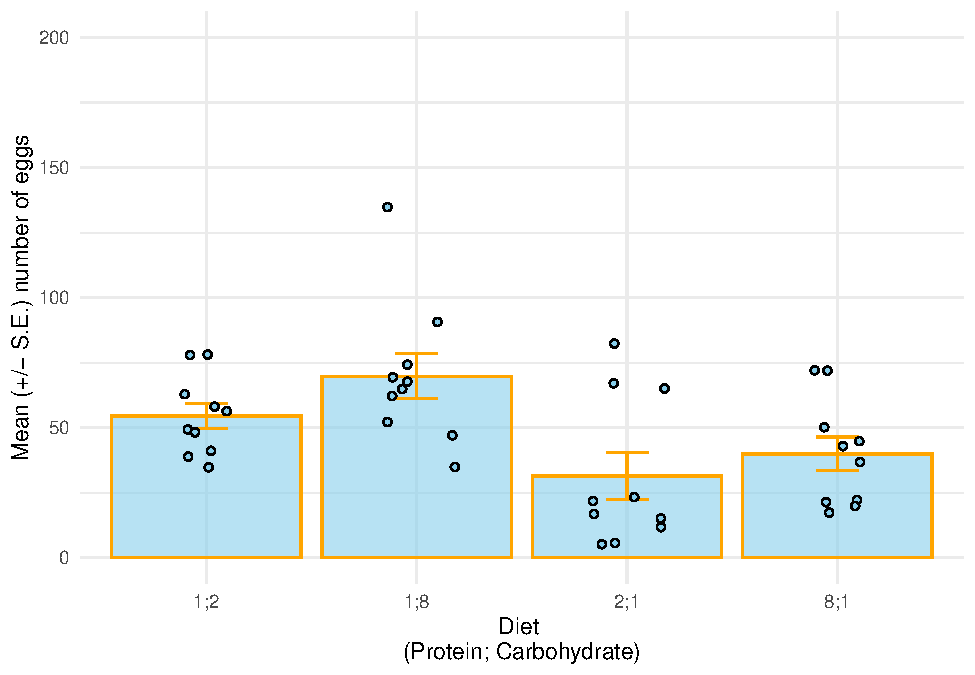
\includegraphics{Experimental-Write-up_files/figure-latex/unnamed-chunk-2-1.pdf}
\textbf{\textbf{Figure 1: A boxplot comparing feeding behaviour of mated
and virgin females.}} Figure shows a plot with the mean average +/- S.E.
of where the mated females preferred to feed (left), compared with a
mean average +/- S.E. of where the virgin females preferred to feed
(right).

The significance of diet on mated and virgin \emph{drosophila
melanogaster} seperatley to look for the signifiance in choosing a
particular diet. For mated females, it was found that there was a
statistically significant difference in choosing a diet high in protein
and low in carbohydrate (8:1) over a diet which was low in protein and
high in carbohydrate (1:2). Post hoc analysis (Tukey test:
z\textsubscript{1151} = -9.065, P \textless{} 0.0001). There was a mean
average of 2.74 +/- S.E. 0.138 flies per patch on an 8:1 diet, and only
a mean average of 0.98 +/- S.E. 0.085 flies per patch on a 1:2 diet.
Emphasising again the significance on a diet which is high in protein
for a mated female.

For virgin females, they were a lot less `choosy' about the diets they
chose to feed and spend time on, although there was a significant
difference found (Tukey test: z\textasciitilde\textasciitilde{} = 4.443,
P 0.0002) between diets 1:8 and 8:1. There was a mean average of 2.55
+/- S.E. 0.128 flies per patch on the 1:8 diet and only a mean average
of 1.64 +/- S.E. 0.146 flies per patch on the 8:1 diet.

\hypertarget{oviposition-behaviour}{%
\subsubsection{Oviposition behaviour}\label{oviposition-behaviour}}

The significance of oviposition preference was tested on both mated and
virgin female \emph{drosophila melanogaster}

The first experiment investigated was looking into mated and virgin egg
count. A generalised linear model was quasipoisson was used to count for
overdispersion, it was found that there was not a significant difference
in the interaction effect between where mated females laid their eggs
and where virgin females laid their eggs (ANOVA: F\textsubscript{3,64} =
0.069, P = 0.9 ), so this factor was not tested in the model.

Looking at the significance of diet choice in mated and virgin female
flies individually showed there was a significant difference in the diet
in which a mated female chose to lay their eggs, investing into protein
and carbohydrate differences, there was a mean average of 121 +/- S.E.
14.1 eggs laid on the 1:8 diet and only a mean average of 4.21 +/- S.E.
1.52 eggs laid on the 8:1 diet, showing a statistically significant
difference (Tukey test: t\textasciitilde\textasciitilde{} = 7.342, P =
\textless{} 0.0001). Investigating the significance into where virgin
females laid their eggs showed there was also a statistically
significant difference in a 1:8 diet and a 8:1 diet (Tukey test:
t\textasciitilde\textasciitilde{} = 4.127, P = 0.0026). With an average
of 74.4 +/- S.E. 17 eggs laid on the 1:8 diet and a mean average of 1.25
+/- 1.25 SE eggs laid on the 8:1 diet.

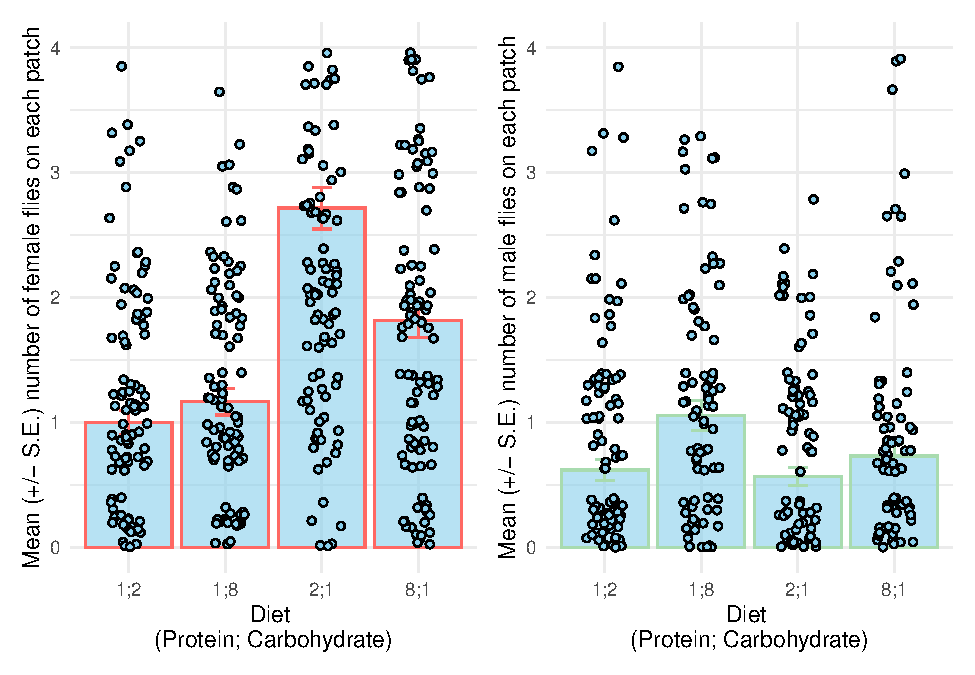
\includegraphics{Experimental-Write-up_files/figure-latex/unnamed-chunk-3-1.pdf}
\textbf{Figure 2: A boxplot showing the eggs counted from mated females
and virgin females.} Boxplot shows the mean average +/- S.E. eggs from
the varying protein: carbohydrate food patches.

The same experiment was repeated, where the oviposition preference of
mated females was investigated. To test for the significance in
oviposition behaviour in the mated females, a linear model was used
with.

It was found that although there was not a lot of differences, there
were significantly more offspring emerging from diets 1:8 than diets 1:2
(t\textasciitilde\textasciitilde{} = 2.379, P = 0.019). Overall there
was a mean average of 114 +/- S.E. 22.5 offspring emerging from 1:8
diets and a mean average of 68.9 +/- 10.6 S.E. offspring emerging from
the 1:2 diets (Figure 3). As these diets are both diets which are `low
in protein' it shows that although there is not a lot of preference for
any particular diets when mated females are laying their eggs. Data for
virgin female egg laying was not collected for this experiment.

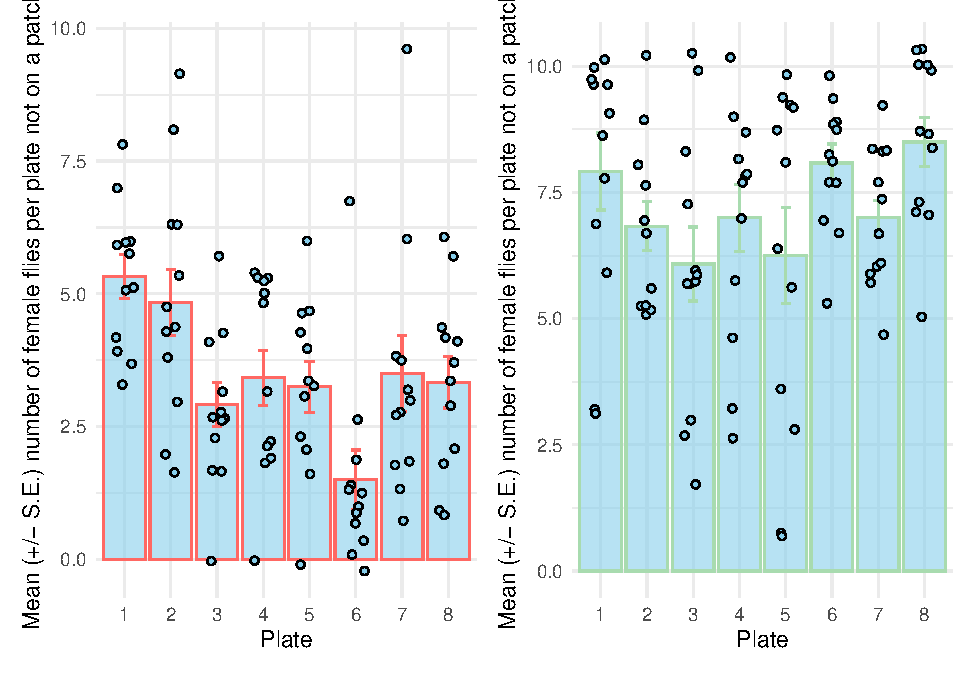
\includegraphics{Experimental-Write-up_files/figure-latex/unnamed-chunk-4-1.pdf}
\textbf{Figure 3: A boxplot of the offspring counted from mated
females.} Boxplot shows mean offspring +/- S.E. that emerged from four
varying protein: carbohydrate diet patches.

Data was also collected in a preliminary experiment, where the egg
counts of where both virgin females and mated females laid their eggs
was collected. It was found that there was no significant differences
found in where virgin females laid their eggs and where mated females
laid their eggs in this experiment. This experiment also showed however,
that there was significantly more eggs laid on the 1:8 diets compared to
the 1:2 diets (P = \textless{} 0.001), with a mean average of 121
+/-13.7 S.E. eggs laid on 1:8, and a mean average of 40.6 +/- S.E. 14.1
laid on the 1:2 diets. There was also a slight significant difference in
eggs laid on the 1:2 diet, and eggs laid on the 8:1 diet (P=0.025), with
a mean average of only 4.21 +/- S.E. 1.52 eggs laid on the 8:1 diets.

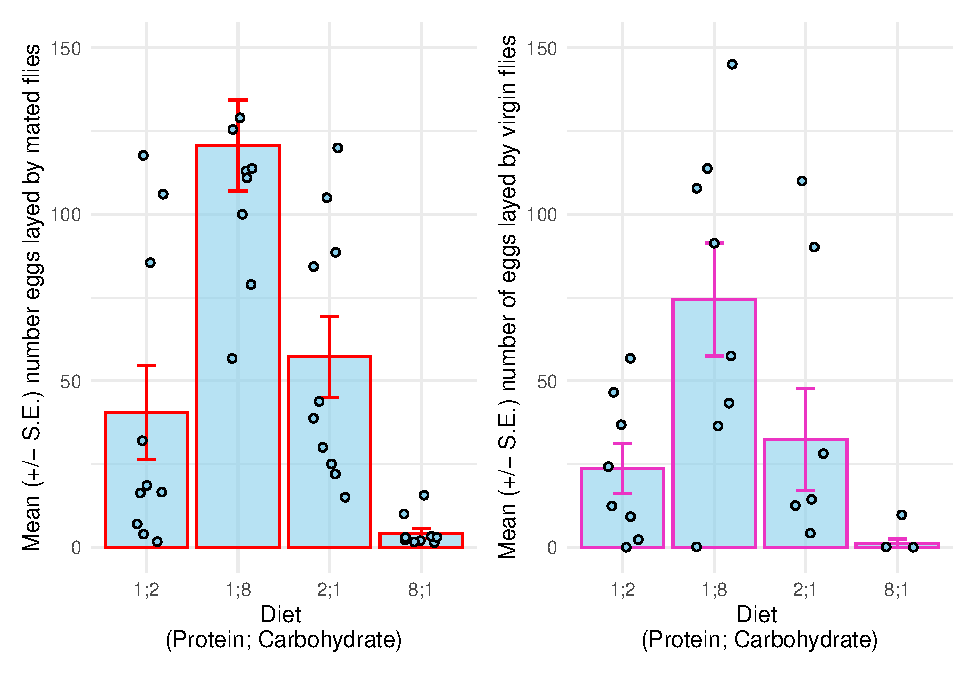
\includegraphics{Experimental-Write-up_files/figure-latex/unnamed-chunk-5-1.pdf}
\textbf{Figure 4: A boxplot showing the eggs counted from mated females
and virgin females.} Boxplot shows the mean average +/- S.E. that
emerged from the varying protein: carbohydrate food patches.

\hypertarget{mated-female-behaviour-alone-vs-mated-female-behaviour-with-males-experiment-3}{%
\subsection{Mated Female behaviour alone vs Mated Female behaviour with
Males (Experiment
3)}\label{mated-female-behaviour-alone-vs-mated-female-behaviour-with-males-experiment-3}}

When looking at female feeding behaviour, and if this changed with
females alone in a feeding assay, to females who were in a feeding assay
with males. There was a small interaction effect of day with diet and
feeding choice, however this was not significant from not having day as
an interaction effect, (F\textsubscript{1,0.91} = 0.941, P = 0.27), and
was therefore dropped from the full model.

A generalized linear model with quasipoisson was used (as there was
over-dispersion), which showed there was no significant difference in
dietary choice between mated females who were alone on a plate and mated
females who were on a plate with males.

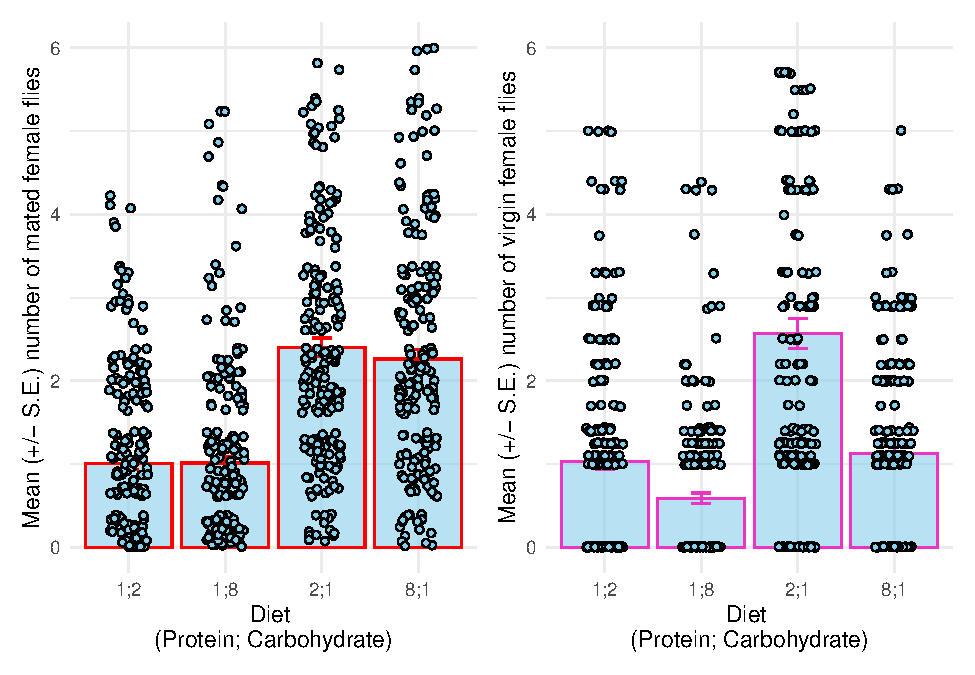
\includegraphics{Experimental-Write-up_files/figure-latex/unnamed-chunk-6-1.pdf}
\textbf{Figure 5: A boxplot showing the feeding behaviour females on a
plate alone and females on a plate with males.} Boxplot shows the mean
average +/- S.E. flies on the varying protein: carbohydrate food patches

\hypertarget{offspring-counts}{%
\subsubsection{Offspring counts}\label{offspring-counts}}

A general linear model was used to test the significance of whether
oviposition preference changed depending on if the mated females were in
a plate alone or in a plate with males. There was no significant
difference found between the diets chosen depending on the conditions
(ANOVA: P = 0.44).

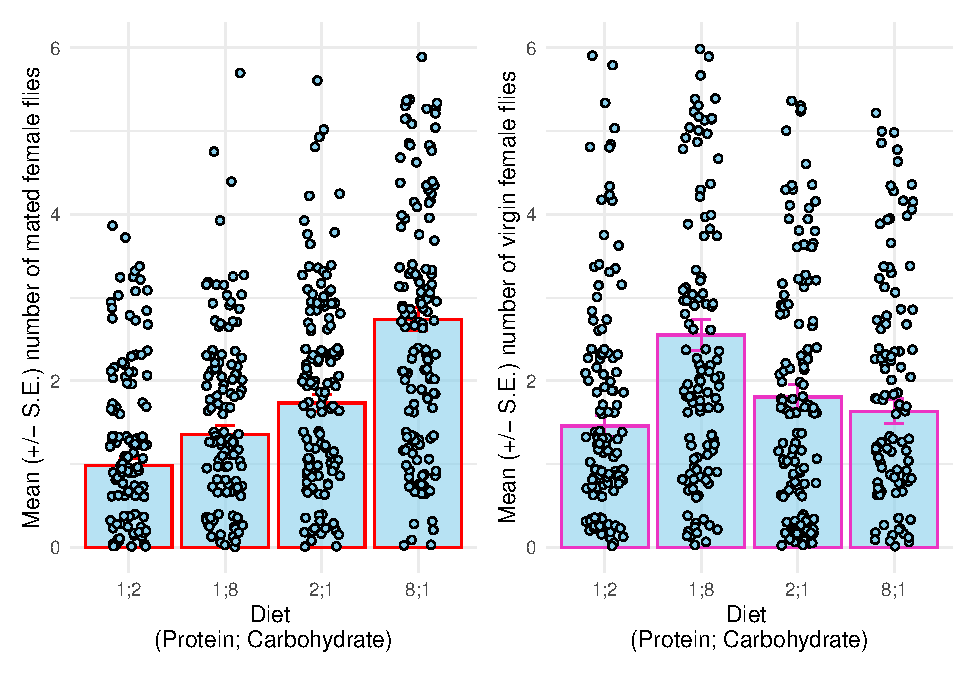
\includegraphics{Experimental-Write-up_files/figure-latex/unnamed-chunk-7-1.pdf}
\textbf{Figure 6: A boxplot showing the offspring count from females in
a plate alone and females in a plate with males.} Boxplot shows the mean
average +/- S.E. of offspring that emerged from the varying protein:
carbohydrate food patches

\end{document}
